\chapter{La struttura della cellula}
\section{La parete cellulare}
Tutti i batteri dispongono di una parete cellulare, la quale assume un ruolo strutturale, conferendo la forma specifica della specie e rigidità, e 
protettivo, ad esempio contro la lisi. Il citoplasma dei batteri infatti contiene un’alta concentrazione di soluti, creando una pressione osmotica 
significativa dell’ordine di 2atm, la stessa delle gomme delle automobili. Lo studio della parete cellulare è stato importante non solo per capire 
ulteriormente i processi vitali di una cellula procariote, ma anche per la sintesi di antibiotici. Molti antibiotici vanno ad agire sulla distruzione della 
parete cellulare ed essendo che le cellule umane ne sono prive, credo un chiaro beneficio nel trattare infezioni batteriche.
\subsection{Peptidoglicano}
\begin{multicols}{2}
\begin{figure}[H]
	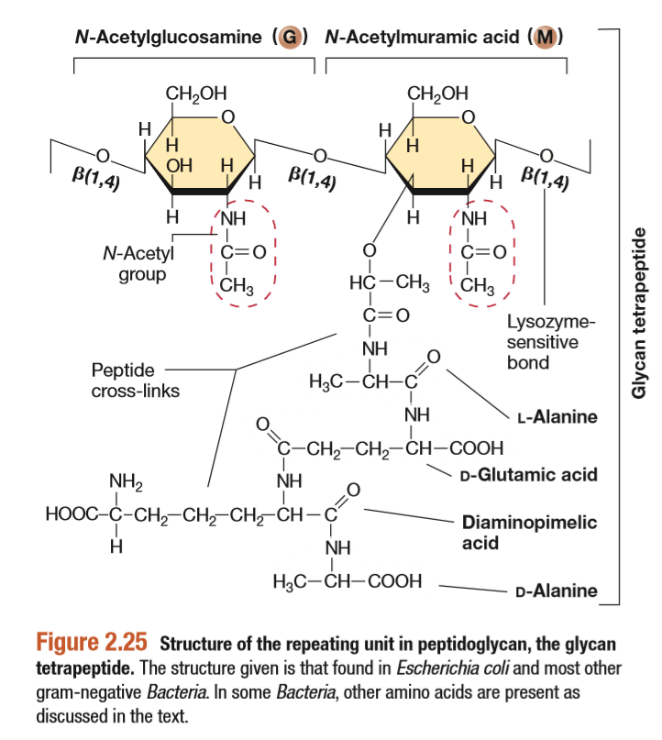
\includegraphics[width=0.5\textwidth]{Pictures/Peptidoglicano.png}
\end{figure}    
\columnbreak
\begin{figure}[H]
	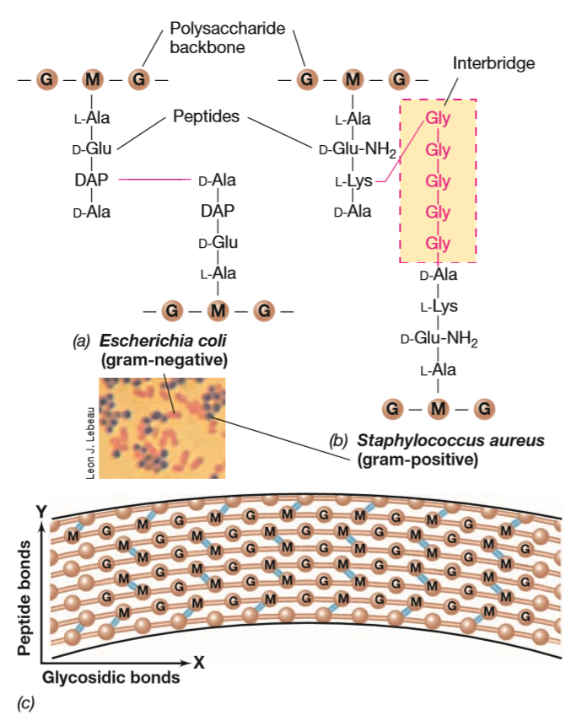
\includegraphics[width=0.5\textwidth]{Pictures/Peptidoglicano2.png}
\end{figure}       
\end{multicols}
La parete cellulare dei batteri possiede uno strato rigido che conferisce rigidità. Questo strato si chiama peptidoglicano o mureina. Il peptidoglicano è un 
polisaccaride composto principalmente da due derivati dello zucchero, N-acetilglucosamina (NAG) e acido N-acetilmuramico (NAM), entrambi strutturalmente 
simili al glucosio. Lunghe catene di peptidoglicano (formate da NAM e NAG covalentemente associate) vengono sintetizzate vicina l’una alle altre, creando un 
foglio che circonda la cellula e sono connesse tra loro da legami crociati di quattro amminoacidi. I quattro amminoacidi solitamente presente sono L-
Alanina, D- Alanina D-Acido glutammico, Acido diamino-pimelico (DAP), che formano legami crociati che, a seconda della specie batterica, possono essere 
diretti o indiretti (ponte peptidico). Nei batteri gram-negativi il legame crociato è formato da un legame peptidico dal gruppo amminico di DAP di una 
catena con il gruppo carbossile dell’ultimo D-Alanina dell’altra catena. Nei batteri gram-positivi invece, il legame spesso avviene tramite un corto ponte 
peptidico il cui numero e tipo di amminoacidi varia da specie a specie. 
\subsection{Parete cellulare nei gram-positivi e gram-negativi}
\begin{wrapfigure}{l}{0.6\textwidth}
  \begin{center}
    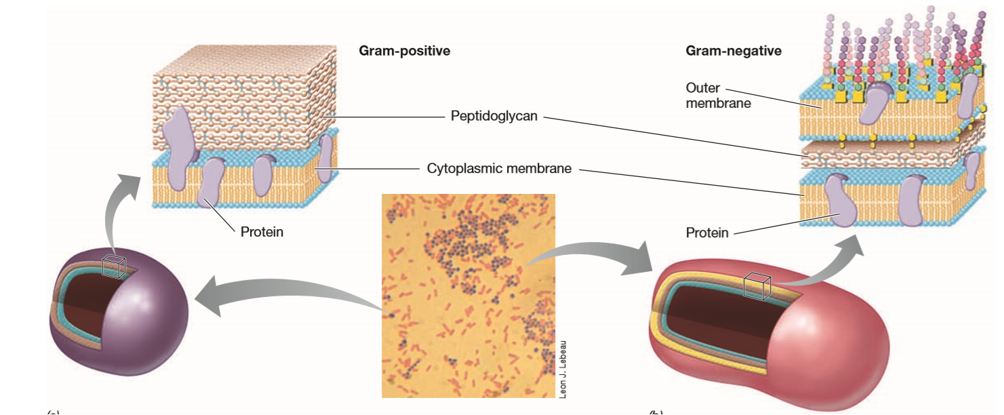
\includegraphics[width=0.58\textwidth]{Pictures/3.png}
  \end{center}
\end{wrapfigure}
Le pareti cellulari nel mondo dei batteri assumono principalmente due strutture diverse, che hanno portato ad una classificazione che consiste nel 
suddividere i microrganismi in gram-positivi e gram-negativi.La colorazione di Gram in breve: The structural differences between the cell walls of gram-
positive and gram-negative Bacteria are responsible for differences in the Gram stain reaction. Recall that in the Gram stain, an insoluble crystal violet–
iodine complex forms inside the cell. This complex is extracted by alcohol from gram-negative but not from grampositive bacteria (Section 2.2). As we have 
seen, gram-positive bacteria have very thick cell walls consisting primarily of peptidoglycan. During Gram staining, the gram-positive cell wall is 
dehydrated by the alcohol, causing the pores in the walls to close and preventing the insoluble crystal violet–iodine complex from escaping. By contrast, in 
gram-negative bacteria, alcohol readily penetrates the lipid-rich outer membrane and extracts the crystal violet–iodine complex from the cell. After alcohol 
treatment, gram-negative cells are nearly invisible unless they are counterstained with a second dye, a standard procedure in the Gram stain
\subsubsection{Parete cellullare nei gram+} 
\begin{wrapfigure}{l}{0.5\textwidth}
  \begin{center}
    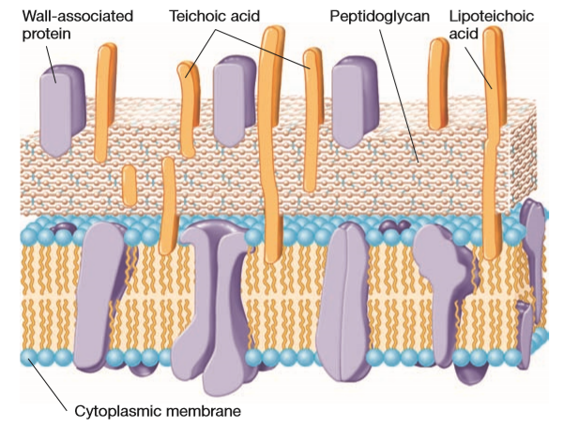
\includegraphics[width=0.48\textwidth]{Pictures/4.png}
  \end{center}
\end{wrapfigure}
La prima differenza che si nota tra le due classificazioni di batteri è la quantità di peptidoglicano che possiedono: i gram+ sono infatti ricoperti da un 
solido strato di mureina che è anche 50 volte più spesso di quello dei gram-, che invece ne hanno solo un piccolo strato chiuso tra due membrane cellulari.
Nei gram-positivi il $90\%$ della parete cellulare e, anche se alcuni batteri ne hanno un solo strato, la maggior parte ha una parete composta da diversi 
“fogli” di peptidoglicano posti l’uni sugli altri. Si pensa che il peptidoglicano sia sintetizzato in “tupi” di 50nm di dimensione, i quali contengono al 
loro interno legami crociati di fili di glicano e man mano che questi tubi vengono sintetizzati, formano legami tra di loro e rendono ancora più stabile la 
struttura. I gram+ hanno sulla loro parete cellullare oltre che a proteine (funzione di trasporto, strutturale?) anche acidi teicoici e lipoteicoici. Il 
termine "acidi teichoici" comprende tutte le pareti cellulari, la membrana citoplasmica e i polimeri capsulari composti da fosfato glicerol o fosfato di 
ribitolo pag73 pdf. Gli acidi teichoici sono legati covalentemente all’acido muramico nella parete. Poiché i fosfati sono caricati negativamente, gli acidi 
teichoici sono in parte responsabili della carica elettrica negativa complessiva della superficie cellulare. Gli acidi teichoici funzionano anche per legare 
Ca2+ e Mg2+ per l'eventuale trasporto nella cellula. Alcuni acidi teichoici sono covalentemente legati ai lipidi della membrana, e questi sono chiamati 
acidi lipoteichoici. Gli acidi lipoteicoici assumono quindi la funzione di ancoraggio della parete alla membrana citoplasmatica.
Anche se la maggior parte dei procarioti non può sopravvivere in natura senza le loro pareti cellulari, alcuni lo fanno. Questi includono i microplasma, 
batteri patogeni legati ai batteri gram-positivi che causano diverse malattie infettive degli esseri umani e di altri animali, e Thermoplasma e simili, 
specie di Archaea che sono naturalmente prive di pareti cellulari. Questi organismi sono in grado di sopravvivere senza pareti cellulari perché contengono 
membrane citoplasmiche insolitamente forti o perché vivono in habitat osmoticamente protetti come il corpo animale. La maggior parte dei microplasma hanno 
steroli nelle loro membrane citoplasmiche, e queste molecole conferiscono forza e rigidità alla membrana, come fanno nelle membrane citoplasmiche delle 
cellule eucariotiche. Anche le membrane dei termoplasma contengono molecole chiamate lipolicani che svolgono una funzione di rafforzamento simile.
\subsubsection{Parete cellullare nei gram-}
\begin{figure}[H]
	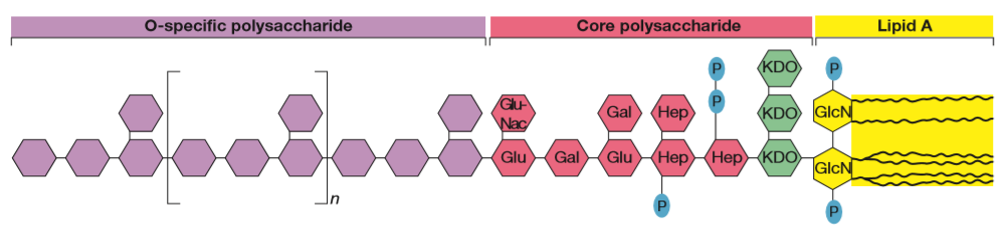
\includegraphics[width=\textwidth]{Pictures/5.png}
\end{figure} 
\newpage
\begin{wrapfigure}{l}{0.5\textwidth}
  \begin{center}
    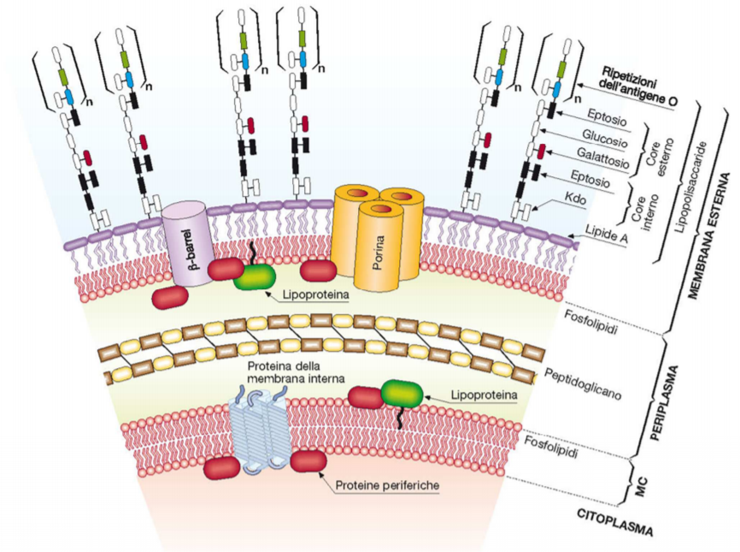
\includegraphics[width=0.48\textwidth]{Pictures/6.png}
  \end{center}
\end{wrapfigure}
La parete cellulare dei gram- è formata principalmente da una membrana esterna, mentre un sottile strato di peptidoglicano si trova in mezzo alle due 
membrane. La membrana esterna non è composta solo da fosfolipidi e proteine come quella citoplasmatica, ma anche da polisaccaride (traduzione), che si 
unisce ai lipidi per formare una struttura complessa. Per questo motivo la membrana esterna viene spesso chiamata strato lipopolisaccaride, o semplicemente 
LPS. Sebbene permeabile a piccole molecole, la membrana esterna è impermeabile alle proteine e ad altre molecole molto grandi. Infatti, una delle principali 
funzioni della membrana esterna è quella di impedire che le proteine le cui attività si verificano al di fuori della membrana citoplasmatica si diffondano 
all’esterno dalla cellula. Queste proteine sono presenti in una regione chiamata periplasma. Questo spazio, situato tra la superficie esterna della membrana 
citoplasmica e la superficie interna della membrana esterna, è largo circa 15 nm. Il periplasma ha una consistenza simile a quella di un gel, dovuta 
all’alta concentrazione di proteine. A seconda dell'organismo, il periplasma può contenere diverse classi di proteine. Questi includono gli enzimi 
idrolitici, che funzionano nella degradazione iniziale delle molecole alimentari; proteine leganti, che iniziano il processo di trasporto dei substrati; e 
chemorecettori, che sono proteine che governano la risposta chemiotaxis. La maggior parte di queste proteine raggiunge il periplasma tramite un sistema di 
esportazione di proteine presente nella membrana citoplasmatica. La membrana esterna è solo in parte impermeabile alle piccole molecole per la presenza di 
proteine chiamate porine, che fungono da canali per l’entrata e l’uscita di soluti. Sono noti diverse porine, tra cui classi specifiche e non specifiche. Le 
porine non specifiche formano canali pieni d'acqua attraverso i quali può passare qualsiasi piccola sostanza. Al contrario, porine specifiche contengono un 
sito di legame per solo una o un piccolo gruppo di sostanze strutturalmente correlate. Strutturalmente, le porine sono proteine transmembrana composte da 
tre sotto unità identiche. Oltre ai tre canali principali che si vengono a formare, nel centro della porina si trova un piccolo foro di circa 1nm di 
diametro attraverso il quale possono viaggiare molecole estremamente piccole. 
\subsection{Lisozima}
\begin{multicols}{2}
\begin{figure}[H]
	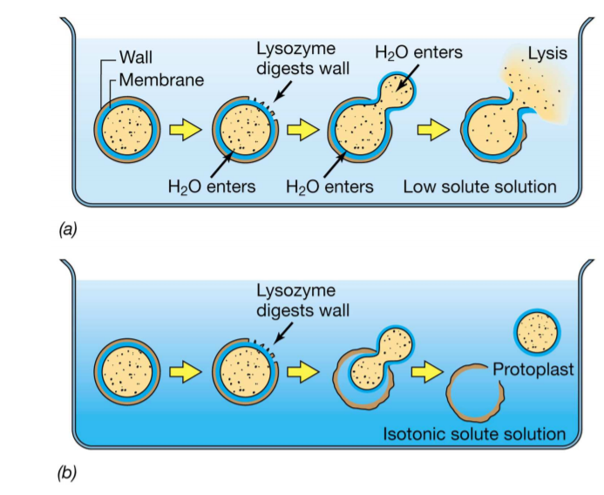
\includegraphics[width=0.5\textwidth]{Pictures/7.png}
\end{figure} 
L’enzima lisozima è una proteina che può rompere i legami $\beta$(1, 4) degli zuccheri NAM-NAG. Protoplasti. 

\begin{itemize}
\item[(a)] In una soluzione diluita (ipotonica) la degradazione della parete con il lisozima rilascia il protoplasto che va incontro a lisi in seguito 
all’ingresso di acqua nella cellula
\item[(b)] In una soluzione isotonica non c’è nessun movimento netto di acqua tra ambiente e protoplasti ed essi rimangono stabili.
\end{itemize}
\end{multicols}
\section{La membrana citoplasmatica}
\begin{figure}[H]
	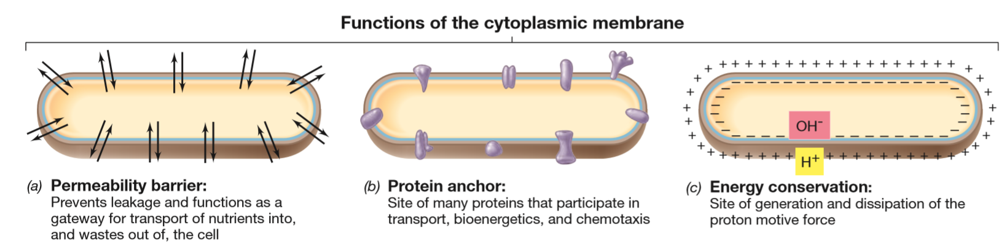
\includegraphics[width=\textwidth]{Pictures/8.png}
\end{figure}
La membrana citoplasmatica circonda il citoplasma e lo separa dall’ambiente. Nel caso in cui la membrana citoplasmatica sia compromessa, l’integrità della 
cellula viene distrutta, il citoplasma si disperde e di conseguenza il batterio muore. La membrana non è così rigida da conferire un’adeguata protezione 
contro la lisi, ma diventa la sua mobilità le permette di impiegarsi nella sua funzione principale: la permeabilità selettiva. Non solo, la membrana funge 
anche da sito di ancoraggio per proteine che sono coinvolte in diverse attività e di conservazione di energia.
\subsection{La struttura}
La struttura generale della membrana è quella di un doppio strato fosfolipidico. I fosfatidi sono composti sia da componenti idrofobici (acidi grassi) che 
idrofili (glicerolo-fosfato) (Figura 2.14). Quando i fosfolipidi si aggregano in una soluzione acquosa, formano naturalmente bistrati. In una membrana 
fosfolipidica, gli acidi grassi puntano verso l'interno verso l'altro per formare un ambiente idrofobico, e le porzioni idrofili rimangono esposte 
all'ambiente esterno o al citoplasma. Gli acidi grassi comuni nella membrana citoplasmatica includono quelli con atomi di carbonio da 14 a 20.
Le membrane citoplasmiche di alcuni batteri sono rafforzate da molecole simili allo sterolo chiamate opanoidi. Gli steroli sono molecole rigide e planari 
che funzionano per rafforzare le membrane delle cellule eucariote, e gli opanoidi svolgono una funzione simile nei batteri.
La membrana contiene inoltre un alto numero di proteine, che hanno tipicamente superfici idrofobe in regioni che attraversano la membrana e superfici 
idrofile in regioni che sono a contatto con l'ambiente e il citoplasma. Molte di esse sono saldamente incorporate nella membrana e sono chiamate proteine 
integrali. Altre hanno una porzione ancorata nelle regioni della membrana e dell'extramembrana che puntano dentro o fuori la cellula. Altre proteine ancora, 
chiamate proteine della membrana periferica, non sono incorporate nella membrana, ma rimangono comunque associate alla sua superfice. Alcune di queste 
proteine periferiche sono le lipoproteine, molecole che contengono una coda lipidica che ancora la proteina alla membrana. Le proteine della membrana 
periferica in genere interagiscono con le proteine integrali della membrana in importanti processi cellulari come il metabolismo energetico e il trasporto. 
Spesso le proteine che devono interagire tra loro in qualche processo sono tipicamente raggruppate in cluster per consentire loro di rimanere adiacenti 
l'una all'altra nell'ambiente semifluido della  membrana.
\begin{multicols}{2}
\begin{figure}[H]
	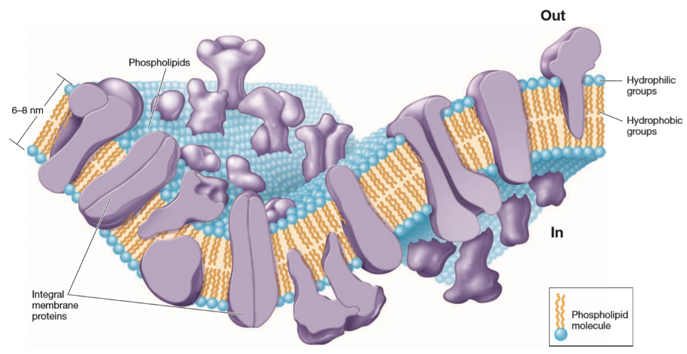
\includegraphics[width=0.5\textwidth]{Pictures/9.png}
\end{figure}
\begin{figure}[H]
	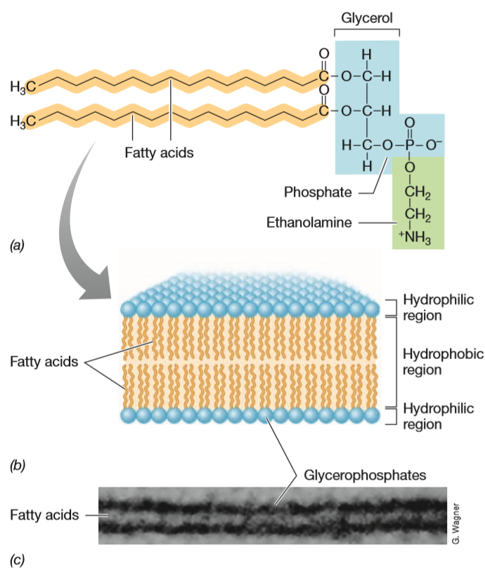
\includegraphics[width=0.5\textwidth]{Pictures/10.png}
\end{figure}
\end{multicols}
\section{Membrana e parete degli archaea}
In contrasto con i lipidi di batteri ed Eukarya in cui ci sono legami estere tra acidi grassi e glicerolo, i lipidi degli Archaea contengono legami etere 
tra glicerolo e le loro catene laterali idrofobiche (catena alifatica). I lipidi degli Archaea mancano quindi di acidi grassi, di per sé, anche se le catene 
laterali idrofobiche svolgono lo stesso ruolo funzionale degli acidi grassi. 
\begin{figure}[H]
	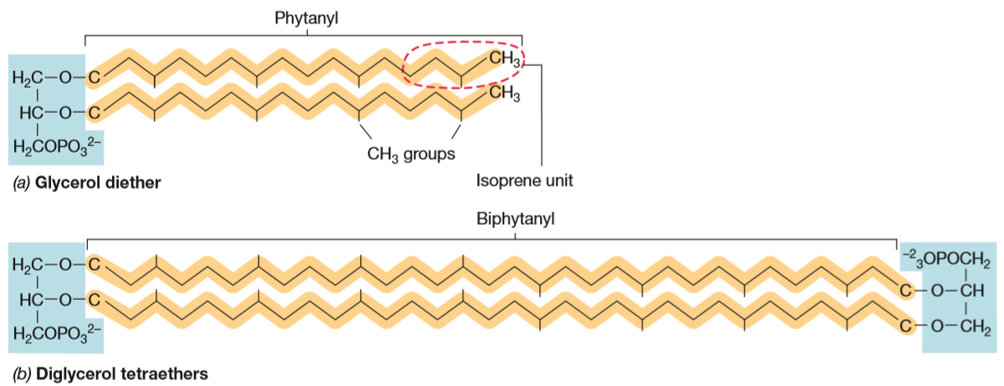
\includegraphics[width=\textwidth]{Pictures/11.png}
\end{figure}
\begin{figure}[H]
	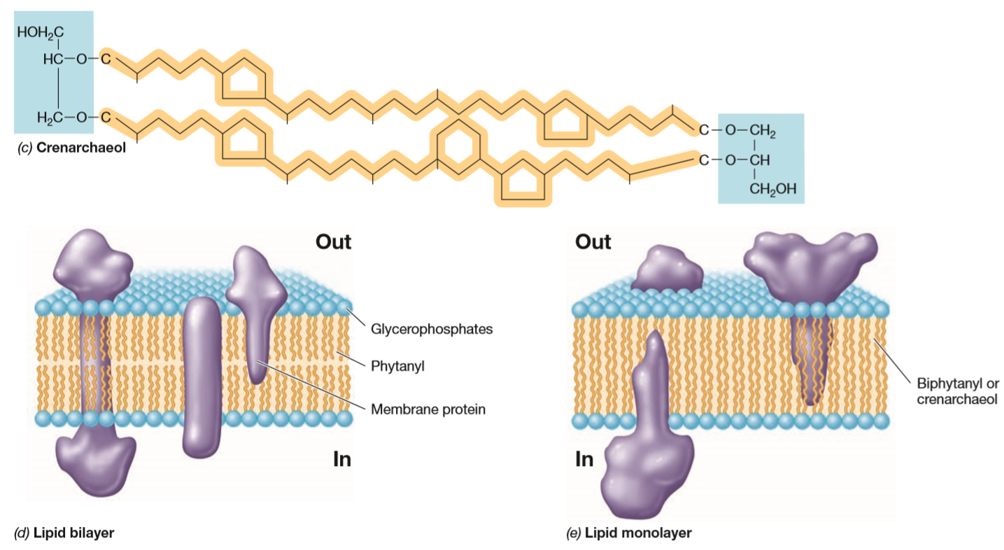
\includegraphics[width=\textwidth]{Pictures/12.png}
\end{figure}
\begin{wrapfigure}{l}{0.5\textwidth}
  \begin{center}
    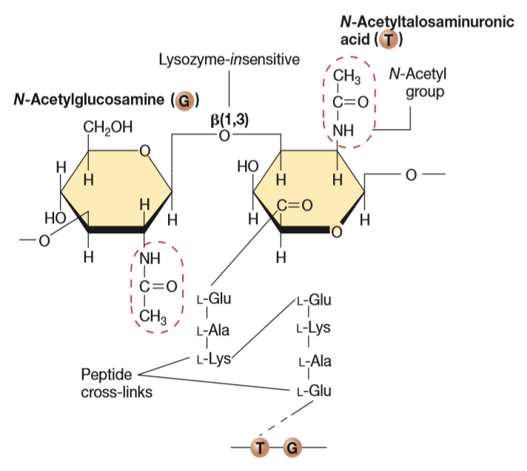
\includegraphics[width=0.48\textwidth]{Pictures/13.png}
  \end{center}
\end{wrapfigure}
Le principali differenze sono le catene isopreniche e il fatto che alcune sono 
a monostrato invece che bistrato. A differenza dei bistrati lipidici, le membrane monostrato lipidiche sono estremamente resistenti al calore e sono quindi 
ampiamente distribuite tra Archaea ipertermofili, organismi che crescono a temperature superiori a 80 gradi centigradi. Esistono anche membrane con una 
miscela di carattere bistrato e monostrato, con alcuni dei gruppi idrofobici opposti covalentmente legati e altri no. Un’altra differenza tra i batteri e 
gli Archaea è la frequente assenza sia di una parete cellullare, sia di una membrana esterna, che vengono sistuititi da una grande varietà di diverse pareti 
cellullari, alcune delle quali hanno delle bio-componenti molto simili a quelle dei batteri, come polisaccaridi, proteine e glicoproteine. Alcuni archaea 
metanogeni (producono metano) hanno una parete costituita da pseudomureina (o pseudopeptidoglicano), costituita da NAG e, al posto di avere il NAM, ha 
l’acido N-acetiltalosaminuronica (NAT). Questo porta ad avere legami $\beta$(1, 3), caratteristica interessante perché li rende insensibili al lisozima e 
all’antibiotico penicillina, che invece nei batteri distruggerebbero il peptidoglicano o ne arresterebbero la sua biosintesi. Alcuni arch/aea non hanno la 
pseudomureina, al suo posto troviamo altri polisaccaridi.
\section{Locomozione microbica}
Molti batteri hanno la capacità di potersi muovere sotto il loro controllo, spesso con l’aiuto di strutture chiamate flagella (flagellum, al singolare) che 
permettono loro di rispondere a degli stimoli ambientali, chiamati tassi (taxes) in biologia. I due principali tipi di movimento sono nuotare e moto a 
scorrimento (glinding). 
\subsection{Il flagello}
\begin{figure}[H]
	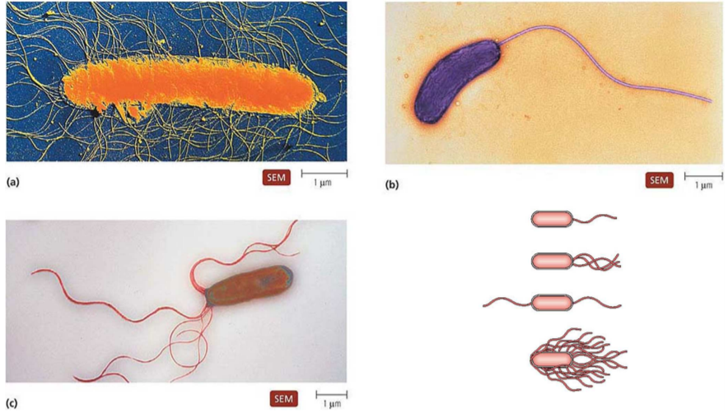
\includegraphics[width=\textwidth]{Pictures/14.png}
\end{figure}

I flagelli batterici sono lunghe e sottili appendici libere da un'estremità e attaccate alla cellula all'altra estremità. I flagelli batterici sono così 
sottili (15-20 nm, a seconda della specie) che un singolo flagello non può essere visto dalla microscopia ottica a meno che non sia macchiato per aumentarne 
il diametro. Tuttavia, i flagelli sono facilmente visibili con il microscopio elettronico. I flagelli si distribuiscono in modo diverso a seconda della 
specie sia per quanto riguarda il numero, che per la posizione. Possono assumere un’organizzazione peritrica (peritrichous) (a) quando numerosi flagelli 
sono distribuiti su tutta la superficie cellulare. Flagelli polari si trovano soltanto alle estremità della cellula (b). L’organizzazione lofotrica 
(lophotrichous) (c) indica la presenza di più di un flagello polare. \\
\newpage
\begin{multicols}{2}
\begin{figure}[H]
	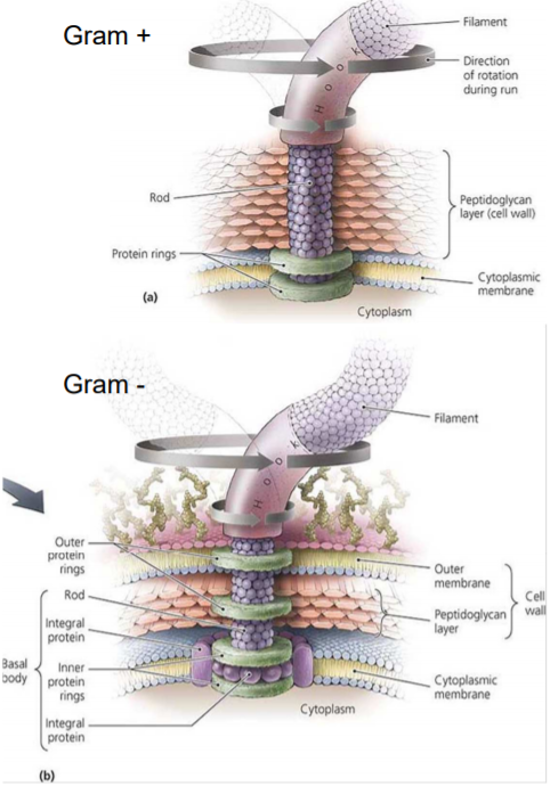
\includegraphics[width=0.48\textwidth]{Pictures/15.png}
\end{figure}
	
\begin{figure}[H]
	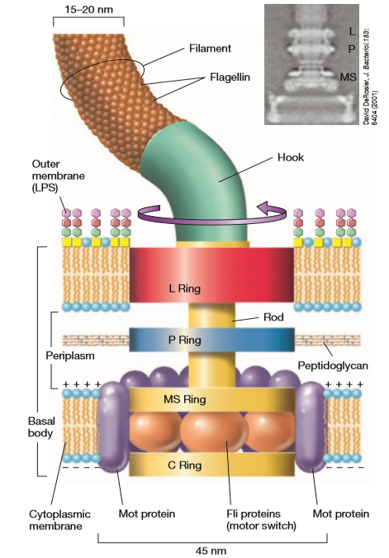
\includegraphics[width=0.48\textwidth]{Pictures/16.png}
\end{figure}
\end{multicols}

Il flagello non è dritto, ma piuttosto un’elica e la distanza tra curve adiacenti è 
costante. Questa wave-lenght è una caratteristica che differisce da specie a specie. Esso è composto principalmente da tre parti: il filamento, l’uncino 
(hook) e la base. Menrte le prime due hanno una composizione chimica e una struttura molto simile tra i vari batteri, la base, o meglio, il modo in cui il 
flagello è ancorato alla parete e alla membrana cellullare cambia a seconda che il batterio sia gram-positivo o gram-negativo. Il filamento è composto da 
molte copie della proteina flagellina. La forma e la lunghezza d'onda del flagello sono in parte determinate dalla struttura della proteina flagellina e in 
una certa misura anche dalla direzione di rotazione del filamento. La sequenza di amminoacidi della flagellina è altamente conservata in specie di batteri, 
suggerendo che la motilità dei flagelli si è evoluta presto e ha radici profonde all'interno di questo dominio. L’uncino è chimicamente diverso dal 
filamento ed è costituito da un solo tipo di proteina. La base è ancorata alla membrana citoplasmatica e alla parete cellulare e possiamo pensare che abbia 
un funzionamento meccanico che assomiglia ad un motore a propellenza di una barca. Il motore consiste in un’asta centrale, chiamata bastoncello, che 
attraversa diversi anelli. Nei batteri gram-positivi, che non hanno una membrana esterna, possiedono solo la coppia di anelli più interna.
 Intorno 
all'anello interno e ancorato nella membrana citoplasmatica c'è una serie di proteine chiamate proteine Mot. Un insieme finale di proteine, chiamate 
proteine Fli, funzionano come l'interruttore del motore, invertendo la direzione di rotazione del flagella in risposta ai segnali intracellulari. Nei 
batteri gram-negativi, un anello esterno, chiamato anello L, è ancorato nello strato di lipopolissaccaride. Un secondo anello, chiamato anello P, è ancorato 
nello strato di peptidoglicano della parete cellulare. Una terza serie di anelli, chiamati anelli MS e C, si trovano rispettivamente all'interno della 
membrana citoplasmatica e del citoplasma.
\subsection{Il movimento flagellare}
\begin{wrapfigure}{l}{0.5\textwidth}
  \begin{center}
    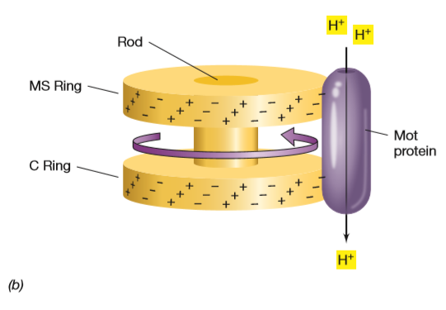
\includegraphics[width=0.48\textwidth]{Pictures/17.png}
  \end{center}
\end{wrapfigure}
Il flagello è un piccolo motore rotativo. Questi motori contengono due componenti principali: il rotore e lo statore. Nel motore del flagello, il rotore è 
costituito dall'asta centrale e dagli anelli L, P, C e MS. Collettivamente, queste strutture costituiscono il corpo basale. Lo statore è costituito dalle 
proteine Mot che circondano il corpo basale e generano momento. La rotazione del flagello è impartita dal corpo basale. L'energia necessaria per la 
rotazione del flagello proviene dallaforza protomotrice. Il movimento dei protoni attraverso la membrana citoplasmica attraverso il complesso Mot, aziona la 
rotazione del flagello e circa 1000 protoni sono traslocati ad ogni rotazione del flagello. In questo modello di turbina protonica, i protoni che scorrono 
attraverso i canali delle proteine Mot esercitano forze elettrostatiche su cariche disposte ad elica sulle proteine del rotore. Le attrazioni tra cariche 
positive e negative causano quindi la rotazione del corpo basale man mano che i protoni scorrono attraverso le proteine Mot.
\subsubsection{Il movimento flagellare nelle diverse categorie}
\begin{wrapfigure}{l}{0.5\textwidth}
  \begin{center}
    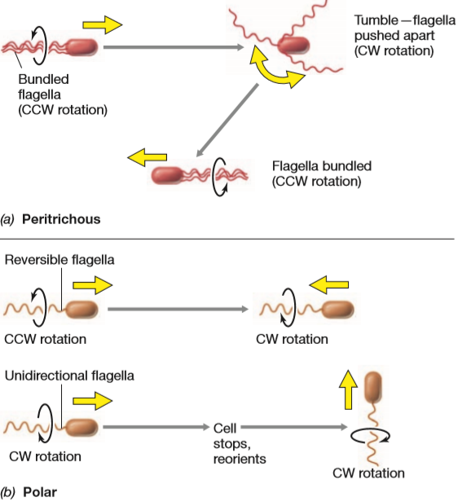
\includegraphics[width=0.48\textwidth]{Pictures/18.png}
  \end{center}
\end{wrapfigure}
Movement in peritrichously and polarly flagellated prokaryotes.  (a) Peritrichous: Forward motion is imparted by all flagella rotating counterclockwise 
(CCW) in a bundle. Clockwise (CW) rotation causes the cell to tumble, and then a return to counterclockwise rotation leads the cell off in a new direction. 
(b) Polar:  Cells change direction by reversing flagellar rotation (thus pulling instead of pushing the cell) or, with unidirectional flagella, by stopping 
periodically to reorient, and then moving forward by clockwise rotation of its flagella. The yellow arrows show the direction the cell is traveling.
\subsection{La sintesi flagellare}
La sintesi del flagello non avviene alla base, come ad esempio i capelli umani, ma dalla punta. Per primo viene sintetizzato l’anello MS ed inserito nella 
membrana citoplasmatica. Successivamente altre proteine di ancoraggio vengono sintetizzate insieme all’uncino, prima che il filamento cominci a formarsi. Le 
subunità di flagellina, sintetizzate nel citoplasma, vengono estruse attraverso un canale di 3 nm all'interno del filamento e si aggiungono alla fine per 
formare il flagello maturo. Un "cap" proteico è presente alla fine del flagello in crescita, che aiuta le molecole di flagellina che si sono diffuse 
attraverso il canale del filamento ad assemblarsi in modo corretto. 
\begin{figure}[H]
	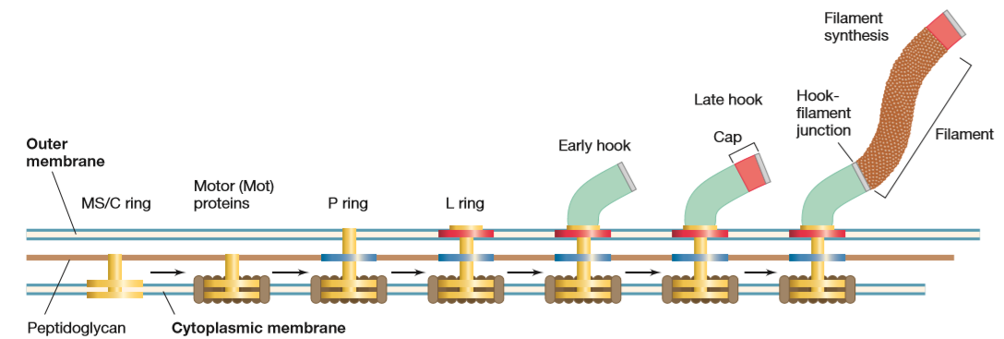
\includegraphics[width=\textwidth]{Pictures/19.png}
\end{figure}
\subsection{I flagelli negli spirocheti}
Nei batteri “spirocheti”, ossia che assumono una forma a spirale, i flagelli sono assiali e si trovano tra la membrana citoplasmatica e quella esterna (sono 
gram-negativi). La rotazione dell’endoflagello porta l’intera cellula a ruotare su se stessa in un movimento elicoidale che consente lo spostamento anche in 
ambienti molto viscosi.
\begin{figure}[H]
	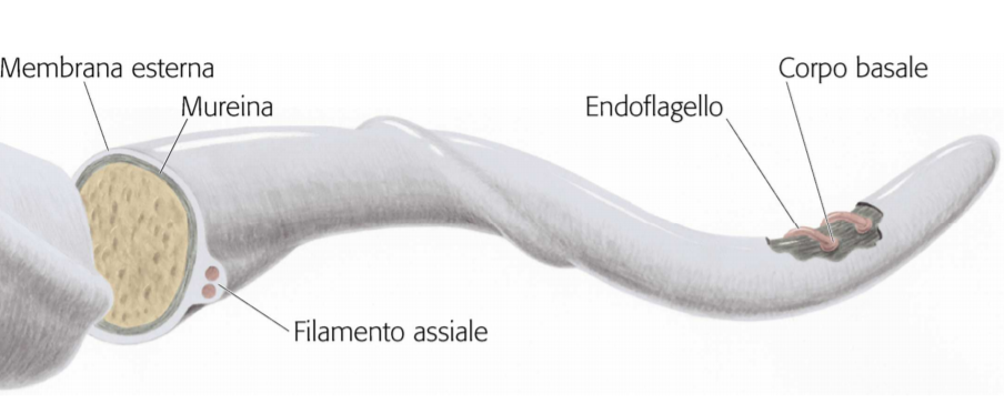
\includegraphics[width=\textwidth]{Pictures/20.png}
\end{figure}